%%%%%%%%%%%%%%%%%%%%%%%%%%%%%%%%%%%%%%%%%%%%%%%%%%%%%%%%%%%%%%%%%%%%%%
% Template Source: Dave Richeson (divisbyzero.com), Dickinson College
% Author: Louis Dod (13bytes.de)
%%%%%%%%%%%%%%%%%%%%%%%%%%%%%%%%%%%%%%%%%%%%%%%%%%%%%%%%%%%%%%%%%%%%%%
% Please report any errors either via pull request, issue (https://github.com/13Bytes/Uni-Merkzettel) or mail (coding@13bytes.de)
% Improvements are also gladly accepted
%%%%%%%%%%%%%%%%%%%%%%%%%%%%%%%%%%%%%%%%%%%%%%%%%%%%%%%%%%%%%%%%%%%%%%


\documentclass[a4paper,10pt,landscape]{article}
\usepackage{fontspec}
\usepackage[T1,EU1]{fontenc}
\usepackage{lmodern}    % font
\usepackage[frenchb]{babel} 
\usepackage{amssymb,amsmath,amsthm,amsfonts}
\usepackage{multicol,multirow}
\usepackage{calc}
\usepackage{ifthen}
\usepackage{mathrsfs}
\usepackage[landscape]{geometry}
\usepackage[colorlinks=true,citecolor=blue,linkcolor=blue]{hyperref}
\usepackage[colorinlistoftodos, ngerman]{todonotes}
\usepackage{xcolor,soul}
\usepackage{cancel}
\usepackage{multirow}
\usepackage{mathabx}
\definecolor{lime}{RGB}{51, 204, 51}
\definecolor{neptune}{RGB}{131,194,188}

\ifthenelse{\lengthtest { \paperwidth = 11in}}
    { \geometry{top=.5in,left=.5in,right=.5in,bottom=.5in} }
	{\ifthenelse{ \lengthtest{ \paperwidth = 297mm}}
		{\geometry{top=.2cm,left=1cm,right=1cm,bottom=.2cm} }
		{\geometry{top=.2cm,left=1cm,right=1cm,bottom=.2cm} }
	}
\pagestyle{empty}
\makeatletter
\renewcommand{\section}{\@startsection{section}{1}{0mm}%
                                {-1ex plus -.5ex minus -.2ex}%
                                {0.5ex plus .2ex}%x
                                {\normalfont\large\bfseries}}
\renewcommand{\subsection}{\@startsection{subsection}{2}{0mm}%
                                {-1explus -.5ex minus -.2ex}%
                                {0.5ex plus .2ex}%
                                {\normalfont\normalsize\bfseries}}
\renewcommand{\subsubsection}{\@startsection{subsubsection}{3}{0mm}%
                                {-1ex plus -.5ex minus -.2ex}%
                                {1ex plus .2ex}%
                                {\normalfont\small\bfseries}}
                                
\newcommand{\OK}{\fcolorbox{black}{lime}{\rule{0pt}{1pt}\rule{1pt}{0pt}}}
\newcommand{\NO}{\fcolorbox{black}{red}{\rule{0pt}{1pt}\rule{1pt}{0pt}}}
\DeclareRobustCommand{\hlcy}[1]{{\sethlcolor{cyan}\hl{#1}}}
\DeclareRobustCommand{\hlgr}[1]{{\sethlcolor{green}\hl{#1}}}
\newcommand{\NDTIME}{\textrm{\textcolor{yellow}{D}\textcolor{orange}{N}TIME}}
\newcommand{\NDSPACE}{\textrm{\textcolor{yellow}{D}\textcolor{orange}{N}SPACE}}
\newcommand{\bbZ}{\mathbb{Z}}
\newcommand{\bbP}{\mathbb{P}}
\newcommand{\bbV}{\mathbb{V}}
\newcommand{\bbE}{\mathbb{E}}
                
\makeatother
\setcounter{secnumdepth}{0}
\setlength{\parindent}{0pt}
\setlength{\parskip}{0pt plus 0.5ex}
% -----------------------------------------------------------------------
\begin{document}

\raggedright
\footnotesize

Merkblatt Theo 3 - Matr.: \hspace{3cm} Name: \hspace{16cm}
{\tiny{\href{https://github.com/13Bytes/Uni-Merkzettel}{\textcolor{gray}{github.com/13Bytes/Uni-Merkzettel}}}}\\

\begin{multicols}{3}
    \setlength{\premulticols}{1pt}
    \setlength{\postmulticols}{1pt}
    \setlength{\multicolsep}{1pt}
    \setlength{\columnsep}{2pt}
    % -----------------------------------------------------------------------

    \section{Master-Theorem}
    \subsection{Master-Theorem I}
    Für $ t(n)= \textcolor{red}{a} \cdot t(\frac{n}{\textcolor{blue}{b}}) +g(n) \quad $ 
    $ = \sum_{i=0}^{\log_b(n)} a^i\cdot g(\frac{n}{b^i})$\\
    Mit $a>0$, $b>1$ und $g\in\Theta(n^{\textcolor{blue}{c}})$: \\
    \begin{tabular}{l|l|l}
     Fall 1 & $\textcolor{red}{a} < \textcolor{blue}{b^c} $  &  $t(n) \in \Theta(n^c) $  \\\hline
     Fall 2 & $\textcolor{red}{a} = \textcolor{blue}{b^c} $  &  $t(n) \in \Theta(n^c \log(n)) $  \\\hline
     Fall 3 & $\textcolor{red}{a} > \textcolor{blue}{b^c} $  &  $t(n) \in \Theta(n^\frac{\log a}{\log b}) $ \hspace*{4bp}\textcolor{gray}{bemerke: $\frac{\log a}{\log b} > c$ }
    \end{tabular}\\

    \hrule
    \smallskip
    
     \subsection{Master-Theorem II}
    $T(n) \leq \sum_{i=1}^{r}T(\alpha_i n) + \mathcal{O}(n) $ \hspace{10bp} für $ \sum_{i=1}^{r} \alpha_i < 1 $\\
    $\Rightarrow T(n) \in \mathcal{O}(n) $
    \hrule
    \smallskip
    
    \section{Ultimate-Heapsort (Median in Linearzeit)}
    - Median aus 5 Elementen ($\frac{n}{5}$ viele Blöcke mit je 6 Vergleichen)\\
    - Median der Mediane\\
    \hspace*{5bp}(rekursiv $\Rightarrow T(\frac{n}{5})$)\\
    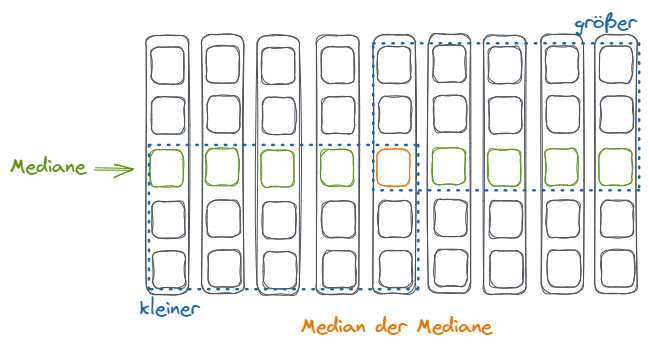
\includegraphics[width=0.18\textwidth]{MedianDerMediane.png}

    $T(n) = \frac{6}{5}n + T(\frac{n}{5}) + n + T(\frac{7}{10}n)$\\
    \textcolor{blue}{$n$: Quicksort-Schritte\\
    $\frac{3}{10}$ können durch Median ausgeschlossen werden}\\
    \textcolor{gray}{bemerke: $\frac{1}{5} + \frac{7}{10} < 1 \ \Rightarrow $ Master-Theorem II $\ \Rightarrow \mathcal{O}(n)$}
    \hrule
    \smallskip

    \section{Euklidischer Algo}
    größter gemeinsamer Teiler \textbf{ggT($m,n$)} \\
    $\textrm{ggT}(n \mod m, m) = \textrm{ggT}(m, m)$
    
    \subsubsection{einfacher Euklid}
    Beispiel $\textrm{ggT}(99,78):$ \hspace*{10bp}
    ${\begin{matrix}\underline {99}&=&1\cdot \underline {78}+\underline {21}\\\underline {78}&=&3\cdot \underline {21}+\underline {15}\\\underline {21}&=&1\cdot \underline {15}+\underline {\ 6}\\\underline {15}&=&2\cdot \underline {\ 6}+\underline {\ 3}\\\underline {6}&=&2\cdot \underline {\ 3}+\underline {\ \textcolor{red}{0}}\end{matrix}}$\\
    Sobald \textcolor{red}{$\textrm{Rest}=0$} ist der Divisor der ggT (hier 3).\\
    \textcolor{gray}{Laufzeit max. $\frac{3}{2}\log_2 m$ Schritte}
    \hrule

    \subsubsection{Erweiterter Euklidischer Algo}
    \textbf{Lemma von Bézout:}  $\textrm{ggT}(m,n) = am+bn $\\
    (ggT immer als Linearkombination darstellbar)
    
    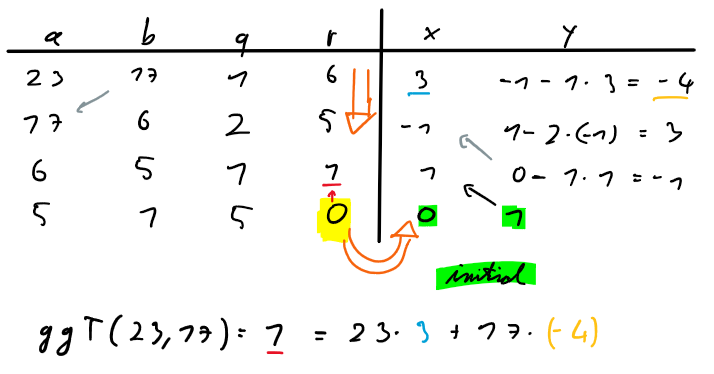
\includegraphics[width=0.21\textwidth]{erwEuklid.png}\\
    Einfachen Euklid ausführen. Danach Spalten x, y von unten füllen.
    \hlgr{Initial ($x=0$, $y=1$).} Danach:\\
    $x_i = y_{i+1}$ \hspace{10bp} und \hspace{10bp}  $y_i = x_{i+1} - (q_i \cdot y_{i+1}) $
    
    Wenn Multiplikative Inverse benötigt zB: $5 \cdot x \equiv 1 \mod 13 $\\
    $\Leftrightarrow 5x \mod 13 = 1 \quad \Longrightarrow \ 13a + 5b = 1$ mit erw. Euklid lösen
    
    \hrule
    \smallskip

    \section{Restklassenring $\bbZ/n\bbZ$}
    beschreibt ''Menge von Mengen''.\\
    Einheitsgruppe $(\bbZ / n\bbZ)^* = \{ k + n\bbZ \ |\ \mathrm{ggT}(k,n)= 1 \}$

    \subsubsection{Wichtigste Eigenschaften}
    $(k+n\bbZ) + (l+n\bbZ) = k+ l +n\bbZ$ (Addition)\\
    $(k+n \bbZ ) \cdot (l+n\bbZ) = k \cdot l + n\bbZ$ (Multiplikation)\\
    $\bbZ / n\bbZ$ ist Körper $\Longleftrightarrow$ $n$ ist prim
    
    \subsubsection{Chinesischer Restsatz}
    Für Teilerfremde Zahlen $m$, $n$:\\
    Abbildung $\varphi:\ \bbZ/ mn\bbZ \rightarrow \bbZ /m\bbZ \times \bbZ / n \bbZ$\\
    \hspace*{48bp} $x + mn\bbZ \mapsto (x+m\bbZ, x+n\bbZ) $ \\
    ist Isomorphismus von Ringen.\\
    \textit{Folgerung: unendlich viele Primzahlen}
    
    \subsubsection{Kleiner Satz von Fermat}
    (Verallgemeinerung von \hl{Satz von Euler}: $ \forall a, n \in \mathbb{N}: \textrm{ggt}(a,n)=1 \ \Longrightarrow$ \hl{$\ a^{\varphi(n)} \equiv 1 \mod n$})
    
    Für Primzahl $p$ und $\forall a \in \mathbb{Z}:\quad a^p \equiv a \mod p$\\
    Falls $p \nmid a \ $ ($a$ kein Vielfaches von $p$): $ \quad a^{p-1} \equiv 1 \mod p$
    
    \vspace{3bp}
    \textbf{Primzahltest (von n) nach Fermat}\\
    Wähle $a \ in \{ 1, ..., n-1\}$ zufällig.\\
    Falls $a^{n-1} \mod n \not\equiv 1 \mod n \quad \Longrightarrow $ n KEINE Primzahl
    \hrule
        
    \subsubsection{Modulo-Tricks}
    - Satz von Euler (für Exponenten) \& Chin. Restsatz (für Modul)\\
    - Satz von Fermat, wenn $\mod p \rightarrow a^{p-1}$ auskl.\\
    - mod 3 ist Quersumme $\mod 3$ \textcolor{gray}{(mod in Summe $\sum a_i \cdot 10^i$ ziehen)}\\
    - binäre Exponentiation\\
    - $x^d\mod n \Leftrightarrow x^{d \mod (p-1)} \mod p \land x^{d \mod (q-1)} \mod q $\\
       \hspace*{1em} mit $p,q$ prim, $n=pq$\\
    - ''$-1$''-Trick
    \hrule
    \smallskip

    \section{RSA}
    Primzahlen $p$ und $q$, $p<q$. Damit $ n=  p \cdot q$, $\ \varphi(n) = (p-1)(q-1) $\\
    Wähle $e > 0$ mit $\textrm{ggT}(e, \varphi(n))= 1$  (Euklidischer Algo)\\
    Berechne $d$: $\ e\cdot d \equiv 1 \mod \varphi(n)$ \hspace*{3bp} \textcolor{gray}{$d < n$}\\
    \hspace*{37bp}\textcolor{gray}{$\Leftrightarrow \ e\cdot d \mod \varphi(n)=1$} bzw. $d=e^{-1} \mod \varphi(n)$
    
    $E(x, (n,e)) = x^e \mod n $ \hspace*{10bp} $(n,e) \in K_{\textrm{pub}}$\\
    $D(y, (n,d)) = y^d \mod n $ \hspace*{10bp} $(n,d) \in K_{\textrm{priv}}$
    \hrule

    \subsection{Eulers $\varphi$-Funktion}
    $\varphi(n) = |\{ k < n: \ \textrm{ggT}(k,n)=1  \}|$\\
    Anzahl ganzer teilerfremde Zahlen unter n.\\
    Für prim: $\varphi(p) = (p-1)$ und  \hl{$\varphi(p^e) = p^{e-1}(p-1)$} \textcolor{gray}{$=p^{e}-p^{e-1}$} 
    \hrule

    \subsection{Primzahldichte}
    $\pi(n)$ Anzahl Primzahlen bis ink. $n$ \hspace{20bp}
    $\pi(n) \geq \frac{n}{\log_2n}$\\
    $\frac{n}{\log_2n} \leq \pi(n) \leq \frac{(2+\epsilon)n}{\log_2n}$
    
    \textbf{Bertrand'sches Postulat}
    $\forall n \geq 1:\ \exists p \textrm{ prim}: \ n < p \leq 2n$
    
    \hrule
    \smallskip
    

    \section{Ungerichtete Graphen $G=(V, E)$}
    $V, E:$ Mengen von Knoten, Kanten. $E \subseteq \binom{V}{2}$
    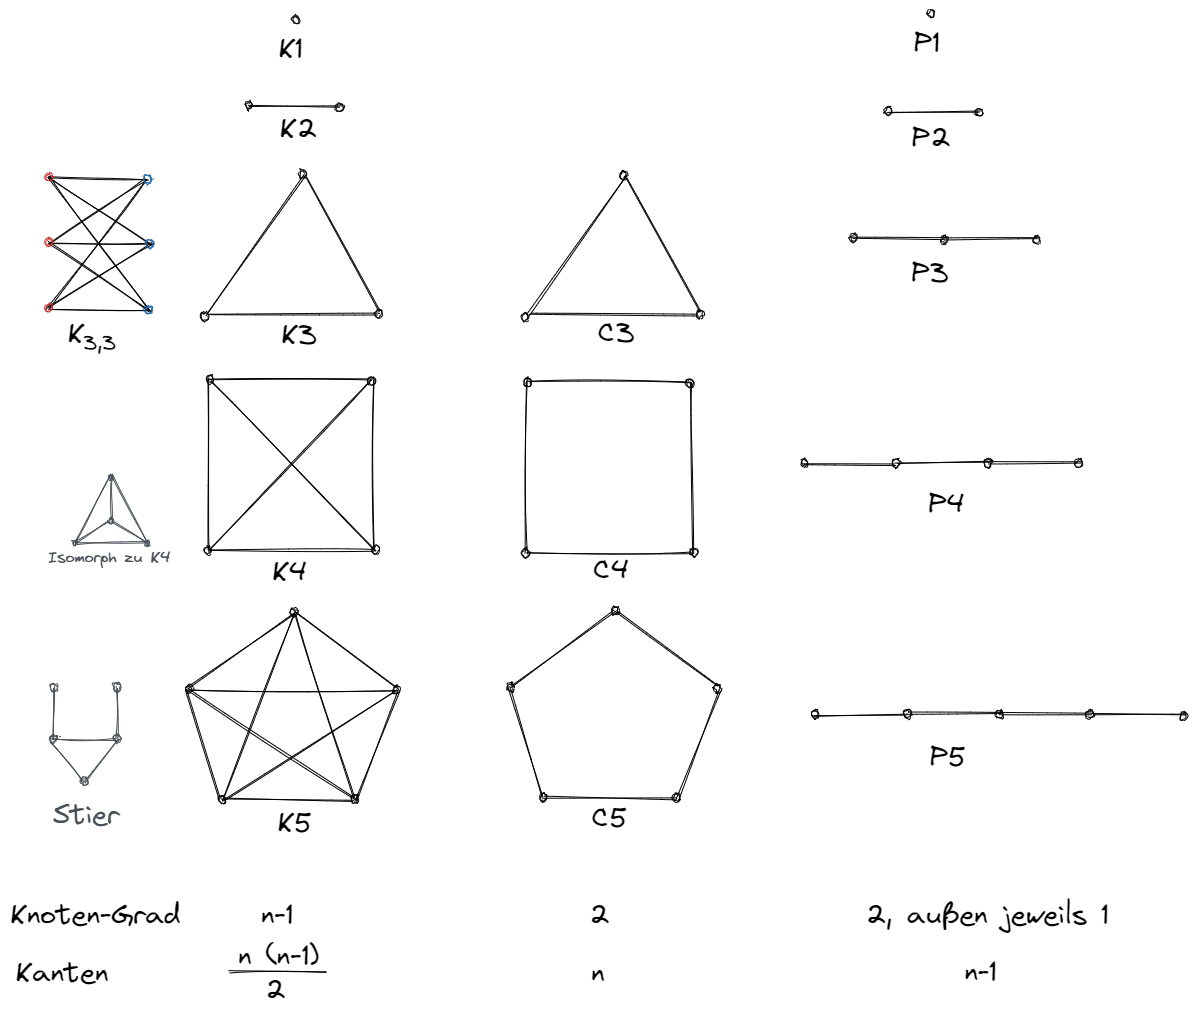
\includegraphics[width=0.30\textwidth]{GraphExport.png}
    \textbf{bipartit:} Knotenmenge $V$ kann in zwei aufgeteilt werden, so dass keine Kante zwei Knoten der gleichen Menge verbindet. Bsp: $K_{3,3}$\\
    \textbf{d(u):} Grad (degrees)\\
    Summe aller Knotengrade ist gerade (ungerichteter Graph).\\
    \textcolor{red}{Anzahl Knoten mit ungeradem Grad ist gerade!}\\
    \textbf{(Perfect) Matching:} So Kanten wählen, dass jeder Knoten mit max. einem anderen Knoten verbunden ist.\\
    Perfect, wenn alle Knoten beteiligt.\\
    \textbf{Unabhängige Menge:} Knoten, die nicht verbunden sind.
    \hrule

    \subsubsection{Clique}
    Graph $G$, 
    $V' \subseteq V$ ist Clique, falls $\forall u,v \in V': \ u\neq v \ \Rightarrow \ (u,v) \in E$\\
    
    \subsubsection{Satz von Ramsey}
    $\forall n: \ \exists N: $ Jeder Graph mit $N$ Knoten hat entweder\\
    \hspace*{37bp} (eine Clique \textcolor{red}{oder} unabhängige Menge) der Größe $n$
    
    Ramsey-Zahl $R(n)$ für kleinsten Graph $N$
    \hrule
    \smallskip
       
    \subsubsection{Planar}
    Isomorpher G. auf Ebene ohne kreuzende Kanten existiert.\\
    G ist planar $\Leftrightarrow$ Untergraph von G enthält keine Unterteilung von $K_5$ oder $K_{3,3}$
    \textcolor{gray}{\char`\~ Satz von Kuratowski}
    \hrule
    
    \subsubsection{Eulerformel}
    $n-m+f = 2$ \hspace*{10bp} n Knoten, m Kanten, f Facetten \textcolor{red}{(+1 Außen)}.\\
    \textcolor{gray}{für endliche, zusammenhängende, planare Graphen. $n\geq 1$}
    
    Mind. 3 Kanten pro Facette, jede Kante max. 2 Facetten: $3f \leq 2m$ \\
    $4f \leq 2m $ bei bipartiten Graphen
    \hrule
    \smallskip
    
    
    \subsubsection{Wege und Kreise}
    Länge von Weg: Kanten!\\
    \textbf{Euler'scher Weg}: Jede Kante einmal in Pfad \textcolor{red}{(max. 2 Knoten mit ungeradem Grad)}\\
    \textbf{Euler'scher Kreis}: Anfangsknoten = Endknoten \textcolor{red}{(jeder Knoten gerader Grad)}\\
    \textbf{Hamilton'scher Weg:} Jeder Knoten einmal
    
    \hrule
    \smallskip
    
    \vfill\null    % ugly fix to achieve formatting - can be removed, if more text is on this page
    
    \columnbreak
    
    \section{Sortieralgos}
    Da entscheidungsbasiert: mind. Laufzeit von $\log(n!) \in \Omega(n \log n)$. Algo durchquert Baum mit $n!$ Blättern.
    \subsubsection{Dykstra}
    Setzte Kosten aller Knoten auf ∞, außer Startknoten (hier 0). \\
    Füge alle Knoten in eine Queue.\\
    
    Wähle Konten mit kleinstem Wert.\\
    -> Setzte Kosten aller ausgehend verbundenen Knoten auf:\\
    \hspace*{10bp} Eigene Kosten + Kosten des Pfades (Wenn niedriger, als die aktuellen)\\
    WIEDERHOLE, bis Queue leer ist.\\
    
    \textit{Beweisbar optimal, Greedy}
    
    \subsubsection{Bekannte Laufzeiten}
    \begin{tabular}{|l|l|l|}
        \hline
        \textbf{Algo}      & \textbf{Worst-Case}         & \textbf{Average-Case} \\ \hline
        Quicksort &  $\mathcal{O}(n^2)$ &  $ 2n \ln n \textcolor{gray}{\ < 1.4 n \log n} $  \\ \hline
        Heapsort &  $2n \log n  + \mathcal{O}(n)$ &  $2n \log n  + \mathcal{O}(n)$  \\ \hline
        Bottom-up Heapsort & $1.5n \log n +o(n \log n) $ &  $n \log n +o(n \log n) $ \\ \hline
    \end{tabular}
    \hrule
    \smallskip
    

    \subsubsection{CYK-Algo}
    \begin{tabular}{|l|l|ll}
    \hline
    Länge & w1   & \multicolumn{1}{l|}{w2}   & \multicolumn{1}{l|}{...} \\ \hline
    1     & T1,1 & \multicolumn{1}{l|}{T2,1} & \multicolumn{1}{l|}{...} \\ \hline
    2     & T2,1 & \multicolumn{1}{l|}{T2,2} &                          \\ \cline{1-3}
    ...   &      &                           &                          \\ \cline{1-2}
    \end{tabular}
    $T_{i,j} = \{A\in V | A \Rightarrow^*_G a_i ...a_{i+j-1}\}$
    \hrule
    \smallskip


    \subsubsection{Algo optimale Klammerung}
    Ähnlich zu CYK. $T_{i,j} = \min_{i\leq m < j}(T_{i,m} + T_{m+1, j} +  n_{i-1}\cdot n_m \cdot n_j)$\\
    Benutzte Technik: Memoization (dyn. Programmieren)
    \hrule
    \smallskip
    
    \section{Wachstum}
    \subsubsection{Landau-Symbole}
    \begin{tabular}{lll}
    $f\in \begin{smallmatrix}\mathcal {O}\end{smallmatrix}(g)$: & $\prec $ & f wächst langsamer als g \\
    $f\in \mathcal{O}$:                                      & $\preceq$ & f wächst nicht (wesentlich) schneller als ... \\
    $f\in \Theta$:                                           & $\asymp  $ & f wächst genauso schnell wie .. \\
    $f\in \Omega$:                                           & $\succeq $ & f wächst nicht (wesentlich) langsamer als .. \\
    $f\in \omega$:                                           & $\succ $ & f wächst schneller als .. \\
    \end{tabular}

    Beweis $f(n) \in \mathcal{O}(b(n))$: $\exists c \exists n_0 \ \forall (n \geq n_0): \ f(n) \leq c \cdot b(n) $
    
    \subsubsection{Bekannte Relationen}
    $\log(n!) \in \Omega(n \log n) $ \hspace{10bp}  (Worst-Case vergleichsbasiertes Sortieren) \\
    $\Theta(1) < \Theta(\log \log n) < \Theta((\log \log n)^2) < \Theta(\log n)  < \Theta(\sqrt{n}) < \Theta(n)< \Theta(n\cdot\log n)< \Theta(n^2)< \Theta(2^n)< \Theta(n!)< \Theta(n^n) < \Theta(2^{n^2})$
    
    \subsubsection{von $n!$ \textcolor{gray}{(für $n\geq 2$)}}
    $(\frac{n}{2})^\frac{n}{2} < n! < n^n $\\
    $\log(n!) \in\Theta(n \log n) $\\
    $e\cdot(\frac{n}{e})^n \leq n! \leq n\cdot e \cdot (\frac{n}{e})^n $\\
    $n!\approx \sqrt{2\pi n} \cdot (\frac{n}{e})^n $ \hspace{40bp} (Stirling-Formel)
    
    % \vspace*{5bp}
    \subsubsection{von Binomialkoeffizient $\binom{n}{k}$}
    Maximal bei $\binom{2n}{n}$ bzw. $\binom{n}{\lfloor \frac{n}{2} \rfloor}$ = $\binom{n}{\lceil \frac{n}{2} \rceil}$\\
    $\sum_k(\frac{n}{k}) = 2^n$ da alle Möglichkeiten.\\
    $\binom{n}{\lfloor \frac{n}{2} \rfloor}$ = $\binom{n}{\lceil \frac{n}{2} \rceil} \ > \frac{2^n}{n}$ \textcolor{gray}{für $n\geq 3$}
    
    \textcolor{gray}{Durchschnittswert $\binom{n}{k}$ ist $\frac{2^n}{n}$}
    \hrule
    \smallskip

    \subsubsection{kgV$(n)$ - Kleinstes gemeinsames Vielfaches}
    $\textrm{kgV}(n) =\textrm{kgV}(2, ..., n)$\\
    \textcolor{gray}{$\textrm{kgV}(5,8) = 40$, da Primfaktorzerlegung $5=5$, $8=2\cdot2\cdot2$.\\
    Alle P-faktoren in ihrer höchsten Anzahl zusammenfassen und aufmultiplizieren.}\\
     $2^{n-1} < \textrm{kgV}(n) \leq n!$\\
     $2^n < \textrm{kgV}(n) \leq 4^{n-1} \quad $ \textcolor{gray}{für $n\geq7$}\\
     
     $m\cdot \binom{n}{m}$ teilt kgV$(n)$
    \hrule
    \smallskip
    
    \section{Kombinatorik / Stochastik}
    \textbf{Zufallsvariable X:}
    $\Omega \mapsto \mathbb{R}$\\
    $X,Y$ sind unabhängig, wenn: 
    $\bbP(X=x \land Y=y) \ =\ \bbP(X=x) \cdot \bbP(Y=y)$

    \textbf{Erwartungswert $\mathbb{E}(X)$}
    $ = \sum_{\omega \in \Omega}X(\omega) \cdot \mathbb{P}(\omega)$

    \textbf{Varianz $\bbV(x)$} $ = \bbE((X-\bbE(X))^2) = \bbE(X^2)-\bbE(X)^2 $
    \hrule

    \subsubsection{Bedingte Wahrscheinlichkeit}
    $\bbP(B | A) = \frac{\bbP(B\cap A)}{\bbP(A)}$ \\
    $\bbP(A | B) = \frac{\bbP(B | A) \bbP(A)}{\bbP(B)}$ \hspace{10bp} Satz von Bayes
    \hrule

    \subsubsection{Markov-Ungleichung}
    $\forall \lambda>0:\ \mathbb{P}(X\geq \lambda \cdot \mathbb{E}(X)) \leq \frac{1}{\lambda}$ \hspace{10bp} \textcolor{gray}{für $\mathbb{E}(X) > 0$, X ist ZV.}
    \hrule

    \subsubsection{Anzahl Ergebnisse}
    \begin{tabular}{ll|ll|}
    \cline{3-4}
    \multicolumn{2}{l|}{Ziehe $k$ aus $n$ Optionen:}          & \multicolumn{2}{l|}{Zurücklegen}                                                          \\ \cline{3-4} 
                                                       &      & \multicolumn{1}{l|}{Ja} & Nein                                                            \\ \hline
    \multicolumn{1}{|l|}{\multirow{2}{*}{Reihenfolge}} & Ja   & $n^k$                   & $\frac{n!}{(n-k)!}= \binom{n}{k}\cdot k! = n^{\underline{k}}$   \\ \cline{2-2}
    \multicolumn{1}{|l|}{}                             & Nein & $\binom{n+k-1}{k}$      & $\binom{n}{k}$                                                  \\ \hline
    \end{tabular}
    \hrule

    \subsubsection{Binomialverteilung}
    $\bbP(X=k) = \binom{n}{k} \cdot p^k \cdot (1-p)^{n-k}$\\
    $\bbE(X) = n \cdot p$, 
    $\bbV(X) = n \cdot p \cdot (1-p)$
    \hrule

    \subsubsection{Geometrische Verteilung \textit{(Wartezeitprobleme)}}
    $\bbP(X=k) = p \cdot (1-p)^{k}$ (erfolg im $k$-ten Versuch)\\
    $\bbE(X) = \frac{1-p}{p}$, 
    $\bbV(X) = \frac{1-p}{p^2}$
    \hrule
    \smallskip

    % \vfill\null    % ugly fix to achieve formatting - can be removed, if more text is on this page
    % \columnbreak
    
    \section{Nice to knows}
    \subsection{Isomorphismus}
    ist ein bijektiver \textbf{Homomorphismus:} \\
    strukturerhaltende Abbildung:\\
    $\varphi: (M_1, \circ_1, e_1) \mapsto (M_2, \circ_2, e_2)$ mit $\varphi(m\circ_1m') = \varphi(m) \circ_2 \varphi(m')$
    \subsection{Injektiv / Surjektiv}
    Für $X \mapsto Y$:\\
    Injektiv (linkseindeutig): jedes y hat höchstens ein x.\\
    Surjektiv (rechtstotal): jedes y hat mind. ein x. (Jedes Element in Bildmenge wird getroffen)
    \hrule
    \smallskip
    
    \subsection{Primzahlzertifikat für $n$}
    $\forall \textrm{ Primzahlen } p: \ n\equiv 1 \mod p: \ \exists a \in \mathbb{Z}$:\\
    $a^{n-1} \equiv 1 \mod n $ und $a^{\frac{n-1}{p}} \not\equiv 1 \mod n$\\
    erste Primzahlen:
    $2, 3, 5, 7, 11, 13, 17, 19, 23, 29, 31, 37, 41, 43, 47, 53, 59, 61, 67, 71, 73, 79,$
    $83, 89, 97, 101, 103, 107, 109, 113, 127, 131, 137, 139, 149, 151, 157, 163, ...$
    \hrule
    \smallskip
    
    \vfill\null   
    \columnbreak
    
    \subsection{Reihen}
    $ \sum_{k=1}^nq^k = \frac{1-q^{n+1}}{1-q}$  \hspace{10bp} geom. Teil-Reihe\\
    $ \sum_{k=1}^\infty q^k = \frac{1}{1-q} \ $ für $|q|<1$ \hspace{10bp} geom. Reihe\\
    $ \sum_{k=1}^\infty kq^{k-1} = \frac{1}{(1-q)^2} \ $ für $|q|< 1$ \hspace{10bp} geom. Reihe abgeleitet\\
    $ \sum_{k=1}^n k = \frac{n(n+1)}{2} $ \hspace{10bp} gaußsche Summenformel\\
    Harmonische Zahl $H_n = \sum_{i=1}^n \frac{1}{i} \approx \ln(n)$
    \hspace{10bp} \textcolor{gray}{$\ln n \leq H_n \leq \ln n + 1$}\\
    \hrule
    \smallskip
    
    \subsection{Logarithmus-Regeln}
    \begin{tabular}{l|l}
    $\log(x \cdot y) = \log x + \log y$  &
    $\log x^n = n \cdot \log x$ \\
    $\log_a x = \frac{\log_b x}{\log_b a}$  &
    $ a^{\log(b)} = b^{\log(a)}$
    \end{tabular}
    \hrule
    \smallskip

        
    \subsection{Binomialkoeffizienten}
    Wie viele $k$-elementige Teilmengen existieren von $[n]$?\\
    $\binom{n}{k} = \frac{n!}{k!(n-k)!} = \binom{n-1}{k} + \binom{n-1}{k-1}$\\
    $\binom{n}{0} = \binom{n}{n} = 1$ \hspace{1em} und \hspace{1em} 
    $\binom{n}{1} = \binom{n}{n-1} = n$ \\
    $\binom{n}{k} = \binom{n}{n-k}$ \hspace{10bp} (symetrisch)\\
    \hrule
    \smallskip
    
    \subsection{Satz von Wilson}
    $(n-1)! \equiv -1 \mod n \ \Leftrightarrow \ n \textrm{ ist Primzahl}$\\
    \hrule
    \smallskip
    
    \subsection{Fibonacci-Zahlen}
    $F_0=0,\ F_1=1,\ F_{n+2}=F_{n+1} + F_{n}$\\
    $F_n \leq 2^n \leq F_{2n}$ oder $(\sqrt{2})^n \leq F_n \leq 2^n$\\
    $\textrm{ggT}(F_m, F_n) = F_{\textrm{ggT}(m,n)} $
    \hrule
    \smallskip
    

    \subsection{Partitionszahlen}
    n Elemente $\rightarrow$ k nichtleere Teilmengen aufteilen. Reihenfolge egal.\\
    $P(n,k) = P(n-1, k-1) + P(n-k, k)$\\
    \textcolor{gray}{$P_{7,3}=4$, da $7=1+1+5=  1+2+4 = 1+3+3=2+2+3$}
    \hrule
    \smallskip

    \subsection{Catalanzahlen}
    \begin{tabular}{l|l}
    $C_n = \frac{1}{n+1}\binom{2n}{n} =  \frac{1}{2n+1}\binom{2n+1}{n} $ & $C_1=1, C_2=2, C_3=5,C_4=14$ \\
    \end{tabular}
    $C_n \sim \frac{4^n}{n \cdot \sqrt{\pi n}}$ \textcolor{gray}{(durch Stirling)}\\
    $C_n$ gibt Anzahl saturierter Binärbäume mit $n$ inneren Knoten an ($n+1$ Blätter)
    \hrule
    \smallskip
    
    \subsection{Dyck-Wörter (Klammerwörter)}
    a: ''(''   \hspace{2bp}   b: '')''\\
    $D_n$ Menge an Dyck-Wörtern mit Länge $2n$ (also $n$ Klammern)\\
    $w\in D_n \textrm{ wenn }\ |w|_a = |w|_b \land (\forall w_{\textrm{prefix}} \textrm{ aus }w:\ |w_{\textrm{pref}}|_a \geq |w_{\textrm{pref}}|_b )$\\
    $|D_n| = C_n$ \textcolor{gray}{für $n\geq 1$}
    \hrule
    \smallskip

    \subsubsection{Induktion}
    IA, IV \& IS.\\
    Für starke Induktion: IV für $m=1,2,...,n$
    \hrule
    \smallskip
    
    \subsection{Algebraische Strukturen}
    Magma: binäre Verknüpfung $ \circ: S \times S \mapsto S$\\
    Halbgruppe: $\circ$ assoziativ:  $(x \circ y) \circ z = x \circ (y \circ z)$ \\
    Monoid: $(S, \circ)$: $\exists$ neutrales Element  $e: \ \forall x\in S: x\circ e = x = e \circ x $ \\
    Gruppe: Jedes Element hat Inverses: $x \circ x^{-1} = e = x^{-1} \circ x $\\
    
    Alle können \textbf{kommutativ} sein ($x\circ y = y \circ x$) \textcolor{gray}{(gilt nicht für Minus)}
    
    \textbf{Äquivalenzklasse: }
    $[x]_\sim  = \{ y  \in M | x \sim y  \}$ bezogen auf Monoid $(M, \circ)$ mit Äquivalenzrelation $\sim$
    
    \textbf{Quotientenmenge:} 
    $M /\sim =  \{ [x]_\sim \ |\ x \in M  \}$
    
    \textbf{Kongruenzrelation falls:} 
    $x \sim x' \land y\sim y' \Rightarrow x \circ y \sim x' \circ y'$
    \hrule
    
    \textbf{Ring:}
    $(R,+, \cdot)$  abelsche (kommutative) Gruppe unter Addition; Halbgruppe unter Multiplikation
    
    \vfill\null    % ugly fix to achieve formatting - can be removed, if more text is on this page

\end{multicols}
\end{document}
